\documentclass{article}
\usepackage{graphicx}
\usepackage{fancyhdr}
\usepackage{listings}

\let\<\textless
\let\>\textgreater

\graphicspath{ {images/} }
\pagestyle{fancy}
\fancyhf{}
\rhead{Bases de datos geoespaciales}
\rfoot{P\'agina \thepage}

\begin{document}
\begin{titlepage}
  \centering
  {\scshape\LARGE Instituto Tecnol\'ogico de Costa Rica \par}
  \vspace{1cm}
  {\scshape\Large Bases de datos geoespaciales\par}
  \vspace{1.5cm}
  {\Large\itshape Alejandro Rojas\par}
  {\Large\itshape Sa\'ul Zamora\par}
  \vfill
  profesor\par
  Kevin Moraga \textsc{}

  \vfill

% Bottom of the page
\end{titlepage}

\section{Bases de datos espaciales}
Las bases de datos espaciales son bases de datos optimizadas para almacenar datos que representan objetos definidos sobre un espacio geom\'etrico y realizar consultas sobre dichos datos. La mayor\'ia de las bases de datos espaciales permiten representar objetos geom\'etricos simples como puntos, lineas y pol\'igonos. Algunas permitan el manejo de estructuras m\'as complejas como objetos 3D, coberturas topol\'ogicas, redes lineares y redes irregulares trianguladas.
Mientras que las bases de datos tradicionales han sido desarrolladas para manejar m\'ultiples tipos de datos num\'ericos y de caract\'eres, dichas bases de datos requieren funcionalidad adicional para procesar datos espaciales eficientemente y generalmente se agregan tipos de datos como \emph{geometry} o \emph{feature} para manejar datos espaciales.

\section{Consultas espaciales}
Consultas espaciales son el tipo de consulta manejada por los sistemas de bases de datos espaciales. Dichas consultas difieren de las no-espaciales en dos aspectos importantes:
\begin{itemize}
  \item Las consultas espaciales usan datos geom\'etricos como puntos, l\'ineas y pol\'igonos.
  \item Estas consultas consideran la relaci\'on espacial entre las geometr\'ias mencionadas.
\end{itemize}

\section{Tipos de consultas espaciales}
Los nombres de funciones para consultas difieren de un sistema a otro. La siguiente lista contiene funciones com\'unmente a\~nadidas a \emph{PostGIS}, el cual es una extensi\'on de PostgreSQL para el manejo de datos espaciales (el t\'ermino \emph{geometry} se refiere a un punto, l\'inea, caja u otra figura de 2 o 3 dimensiones):

\begin{itemize}
  \item Distance(geometry, geometry) : number
  \item Equals(geometry, geometry) : boolean
  \item Disjoint(geometry, geometry) : boolean
  \item Intersects(geometry, geometry) : boolean
  \item Touches(geometry, geometry) : boolean
  \item Crosses(geometry, geometry) : boolean
  \item Overlaps(geometry, geometry) : boolean
  \item Contains(geometry, geometry) : boolean
  \item Length(geometry) : number
  \item Area(geometry) : number
  \item Centroid(geometry) : geometry
\end{itemize}

\section{Bases de datos geoespaciales}
Una base de datos geoespacial es una base de datos que almacena datos geogr\'aficos, tales como pa\'ises, divisiones administrativas, ciudades e informaci\'on relacionada. Dichas bases de datos pueden ser \'utiles para sitios web que deseen identificar la ubicaci\'on de sus visitantes con el fin de personalizar m\'as la visita.

\section{Caracter\'isticas de las bases de datos espaciales}
Los sistemas de bases de datos usan \'indices para buscar r\'apidamente valores y la forma en la que la mayor\'ia de sistemas indexan la informaci\'on no es \'optima para consultas espaciales. En lugar de eso, las bases de datos espaciales utilizan \'indices espaciales para acelerar las operaciones de base de datos.

Adicionalmente a las consultas t\'ipicas de SQL como \emph{SELECT}, las bases de datos espaciales pueden realizar una amplia variedad de operaciones espaciales:

\begin{itemize}
  \item Medidas espaciales: procesa largo de l\'ineas, \'areas poligonales, distancias entre geometr\'ias, etc.
  \item Funciones espaciales: modificar las caracter\'isticas existentes de un objeto para crear nuevas, por ejemplo, agregando un buffer alrededor de un objeto, etc.
  \item Predicados espaciales: permite consultas de falso\/verdadero sobre relaciones entre objetos, como la superposici\'on de un objeto sobre otro, la ubicaci\'on de un punto dentro de un \'area.
  \item Constructores geom\'etricos: creaci\'on de nuevas geometr\'ias, usualmente mediante la especificaci\'on de los v\'ertices que definen la figura.
  \item Funciones de observaci\'on: consultas que retornan informaci\'on espec\'ifica sobre una figura, como la ubicaci\'on del centro de un c\'irculo.
\end{itemize}

Algunas bases de datos soportan solo versiones simplificadas o modificadas de estas operaciones, especialmente en casos como los de sistemas NoSQL como MongoDB y CouchDB.

\section{\'Indices espaciales}
Los \'indices espaciales son los utilizados por las bases de datos espaciales para optimizar las consultas. Los \'indices convencionales no manejan las consultas espaciales de forma eficiente, tales como que tan lejos est\'a un punto de otro o si todos los puntos caen dentro de un \'area determinada. Los m\'etodos de indexaci\'on espacial m\'as com\'unes incluyen:

\begin{itemize}
  \item R-tree: m\'etodo preferido para la indexaci\'on de datos espaciales. Los objetos (formas, l\'ineas y puntos) son agrupados usando un \emph{rect\'angulo de enlace m\'inimo} o MBR por sus siglas en ingl\'es (\emph{Minimum Bounding Rectangle}). Los objetos se agregan al MBR dentro del \'indice, lo que lleva a que su tama\~no aumente de forma m\'inima.
  \item HHCode
  \item Grid
  \item Z-order
  \item Quadtree
  \item Octree
  \item UB-tree
  \item R+ tree
  \item R* tree
  \item Hilbert R-tree
  \item X-tree
  \item kd-tree
  \item m-tree
  \item M\'etodo de punto de acceso (\emph{Point access method})
  \item Particionamiento espacial binario o BSP-tree por sus siglas en ingl\'es \emph{Binary space partitioning}: subdividir el espacio en hiperplanos.
\end{itemize}

\begin{figure}[!ht]
  \caption{Ejemplo de R-tree para rect\'angulos bidimensionales}
  \centering
    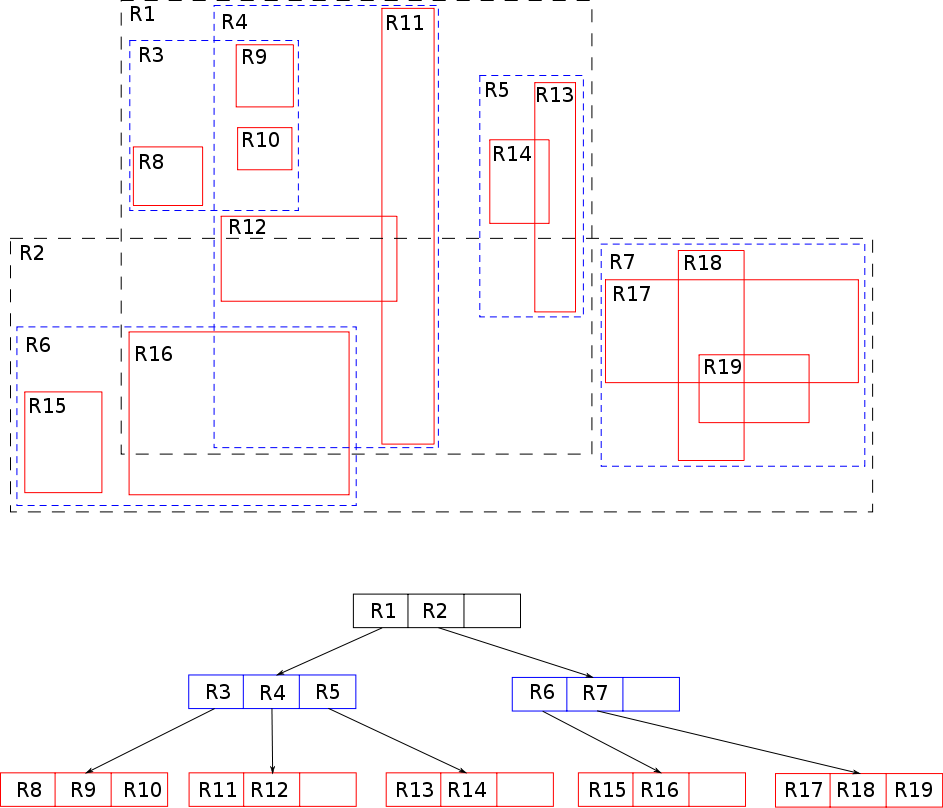
\includegraphics[width=0.4\textwidth]{r-tree.png}
\end{figure}

\begin{figure}[!ht]
  \caption{Visualizaci\'on de un R*-tree para puntos 3D}
  \centering
    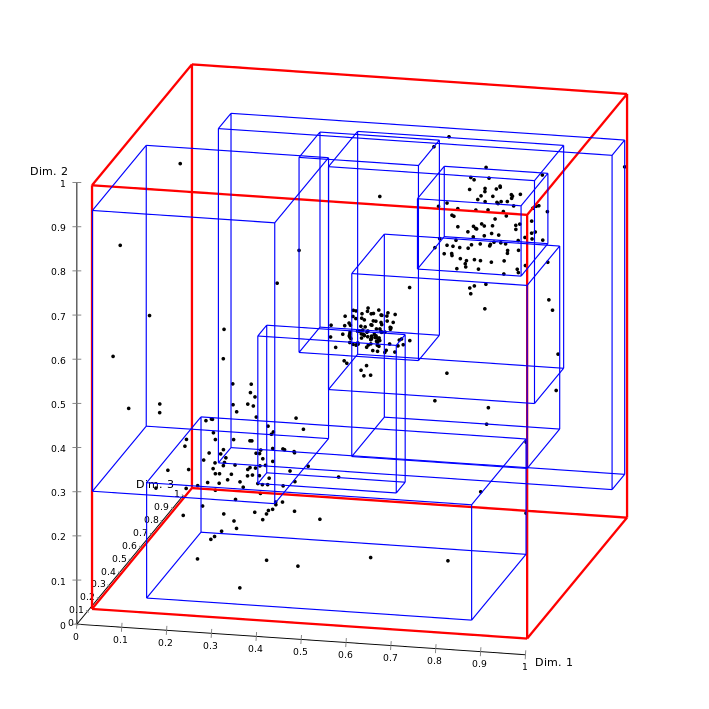
\includegraphics[width=0.4\textwidth]{3d-r-tree.png}
\end{figure}

\section{Usos de las bases de datos espaciales}
Uno de los usos m\'as populares para las bases de datos espaciales son los sistemas de informaci\'on geogr\'afica o GIS (por sus siglas en ingl\'es \emph{Geographic Information Systems}) son sistemas dise\~nados para capturar, almacenar, manupular, analizar, manejar y presentar datos espaciales o geogr\'aficos.

Estas aplicaciones permiten a los usuarios crear consultas interacticas, analizar informaci\'on espacial, editar datos en mapas y presentar los resultados de todas estas operaciones.

En los \'ultimos a\~nos han proliferado sistemas de libre uso con f\'acil acceso a software de mapeo, tales como OpenStreetMap. Dichos servicios dan al p\'ublico acceso a enormes cantidades de datos geogr\'aficos. Otros servicios, como Google Maps, ofrecen al usuario APIs para crear aplicaciones m\'as personalizadas, con diferentes opciones de lincencias para uso comercial.

\section {Prototipo de Sistema de Informaci\'on Geogr\'afica}

La principal caracter\'istica de un SIG es que est\'a dise\~nado para trabajar con datos referenciados con respecto a coordenadas espaciales o geogr\'aficas as\'i como trabajar con distintas bases de datos de manera integrada, permitiendo generar informaci\'on gr\'afica (mapas) \'util para la toma de decisiones. Estos mapas ayudan a condensar varios aspectos de la realidad de una zona, con el objetivo de reconocer la existencia de patrones espaciales sobre alg\'un fen\'omeno de inter\'es. \cite{gisimp} Para generar estos mapas es necesario considerar algunos aspectos b\'asicos:

\begin{itemize}
\item  En primer lugar, comprender la interrogante a la cual se desea dar respuesta con la creaci\'on de un mapa, ya que al entender mejor el problema ser\'a m\'as sencillo determinar que an\'alisis ser\'an necesarios.

\item  Para resolver la interrogante planteada es necesario obtener datos fiables y sobre todo que sean adecuados para nuestros objetivos. Hay que considerar que los datos correspondan con toda el \'area de inter\'es y se tenga toda la información que sea de utilidad para la toma de decisiones.

\item  Es importante generar un diagn\'ostico de los datos para conocer el tipo de informaci\'on que se ha obtenido, la distribuci\'on en la que se encuentra y de ser necesario ordenarla de acuerdo a nuestras necesidades para as\'i dise\~nar o establecer una metodolog\'ia del an\'alisis.

\end{itemize}

Para el desarrollo de este prototipo se utiliz\'o Open Street Map como fuente de datos, adem\'as de tres herramientas de gesti\'on de SIGs, explicadas a continuaci\'on, todas de codigo abierto y disponibles para su descargar en los links referenciados en la bibliograf\'ia \cite{qgis} \cite{geoserver} \cite{leaflet}. Debido a que cada herramienta est\'a debidamente documentada en sus sitios respectivos, se omitir\'a lo relacionado a instalaci\'on y configuraci\'on de cada una, explicando \'unicamente la utilidad que presenta dentro del contexto de un SIG y de este prototipo. 

\subsection {Open Street Maps}

OpenStreetMap (tambi\'en conocido como OSM) es un proyecto colaborativo para crear mapas libres y editables. Los mapas se crean utilizando informaci\'on geogr\'afica capturada con dispositivos GPS m\'oviles, ortofotograf\'ias y otras fuentes libres. Esta cartograf\'ia, tanto las im\'agenes creadas como los datos vectoriales almacenados en su base de datos, se distribuye bajo licencia abierta Licencia Abierta de Bases de Datos (en inglés ODbL). \cite{osmwiki} Para efectos de este prototipo se utilizara la informaci\'on relevante a la zona de Alajuela, Costa Rica.

\subsection {QGIS}

QGIS (anteriormente llamado Quantum GIS) es un Sistema de Informaci\'on Geogr\'afica de código libre para plataformas GNU/Linux, Unix, Mac OS, Microsoft Windows y Android. Este permite manejar formatos raster y vectoriales a través de las bibliotecas GDAL y OGR, así como bases de datos. \cite{qgiswiki} Algunas de sus características son:
\begin{itemize}
\item Soporte para la extensi\'on espacial de PostgreSQL, PostGIS.
\item Manejo de archivos vectoriales Shapefile, ArcInfo coverages, Mapinfo, GRASS GIS, etc.
\item Soporte para un importante n\'umero de tipos de archivos raster (GRASS GIS, GeoTIFF, TIFF, JPG, etc.)
\end{itemize}
QGIS posee un sistema de componentes o plugins que permiten realizar una extensa gama de operaciones sobre datos geogr\'aficos, sin embargo, nos interesa una en particular llamada QuickOSM la cual nos permite extraer informaci\'on directamente de OpenStreetMap aplicando una consulta con la categor\'ia y la zona donde queremos trabajar. OpenStreetMap maneja un sistema de etiquetas mediante pares Llave-valor, por ejemplo, Key: Amenity y Value: Hotels, buscar\'ia la informaci\'on correspondiente a comodidades, especificamente hoteles, que se encuentren en la zona especificada. 

\subsection {GeoServer}
GeoServer es un servidor de c\'odigo abierto escrito en Java. Permite a los usuarios compartir y editar datos geospaciales. Dise\~nado para la interoperabilidad, publica datos de las principales fuentes de datos espaciales usando est\'andares abiertos.\cite{geoserver} Este pretende operar como un nodo a trav\'es de una Infraestructura de Datos Espaciales libre y abierta para ofrecer datos geoespaciales, tal y como ha hecho Apache HTTP Server ofreciendo un servidor web abierto y libre para publicar HTML.\newline
Este tendr\'a la funci\'on de conectarse a la base de datos de PostGIS y enviar las consultas realizadas por el usuario, as\'i como mostrar los datos correspondientes que devuelva la base de datos.

\subsection {Leaflet}

Leaflet es una librer\'ia JavaScript opensource para crear mapas interactivos en un entorno m\'ovil.\cite{leaflet}. Algunas de las ventajas de la API de Leaflet son:
\begin{itemize}
\item Facilidad de uso
\item Soporte tanto a navegadores web como a dispositivos mobiles.
\item API bien documentada
\end{itemize}
Finalmente utilizaremos la librer\'ia Leaflet para mostrar los datos de manera interactiva y atractiva para el usuario, ademas de brindar soporte de capas (layers) las cuales pueden ser removidas y agregadas a necesidad.

\section {Posibles Aplicaciones}
Los Sistemas de Informaci\'on Geogr\'afica no solo permiten mostrar informaci\'on, si no tomar decisiones y acciones en base a esta, un ejemplo de una posible aplicacion consistir\'ia en la creaci\'on de un SIG que permita a los usuarios de Costa Rica buscar disponibilidad acerca de servicios de salud, medicos, fisioterapeutos, entre otros. Esto es, supongamos que se desea obtener una cita con un dentista en una zona en particular del pa\'is, para un d\'ia y un rango de horas especificas, el SIG podr\'ia filtrar la informaci\'on de cl\'incas dentales para verificar cuales de estas tienen disponibilidad en ese horario para atender a un cliente. Adem\'as, podr\'ia permitir al usuario realizar la solicitud de la cita inmediatamente, y el mismo sistema se encargar\'ia de comunicar los datos del cliente a la cl\'inica, acelerando procesos usualmente tediosos y beneficiando tanto a los usuarios que necesitan de atenci\'on m\'edica, como a los centros de servicios de salud que deseen aumentar su clientela.

\newpage

\begin{thebibliography}{99}
\bibitem{spatialdb}  En.wikipedia.org. (2017). Spatial database. [online] Available at: \texttt{https://en.wikipedia.org/wiki/Spatial\_database}

\bibitem{rtree} En.wikipedia.org. (2017). R-tree. [online] Available at: \texttt{https://en.wikipedia.org/wiki/R-tree}

\bibitem{gis} En.wikipedia.org. (2017). Geographic information system. [online] Available at: \texttt{https://en.wikipedia.org/wiki/Geographic\_information\_system}

\bibitem{osmwiki}  En.wikipedia.org  (2017). OpenStreetMap. [online] Available at: \texttt {https://en.wikipedia.org/wiki/OpenStreetMap}

\bibitem{osm} OpenStreetMap. (2017). OpenStreetMap. [online] Available at: \texttt{https://www.openstreetmap.org/\#map=15/10.0131/-84.2072}

\bibitem{qgis} Qgis.org. (2017).  Bienvenido al proyecto QGIS!. [online] Available at: \texttt{ https://www.qgis.org/es/site/index.html}

\bibitem{geoserver} Geoserver.org. (2017).  GeoServer. [online] Available at: \texttt{http://geoserver.org/}

\bibitem{leaflet} Leafletjs.com. (2017). Leaflet — an open-source JavaScript library for interactive maps. [online] Available at: \texttt{http://leafletjs.com/index.html}

\bibitem{gisimp}  Gulfprogram.ucsd.edu.. (2017).   Importancia de los Sistemas de Informaci\'on Geogr\'afica (SIG) en la Conservaci\'on. [online] Available at: \texttt{http://gulfprogram.ucsd.edu/blog/coastal-and-marine/importancia\-de-los-sistemas-de-informacion-geografica-sig-en-la-conservacion/}

\bibitem{qgiswiki}  Es.wikipedia.org  (2017). QGIS. [online] Available at: \texttt {https://es.wikipedia.org/wiki/QGIS}

\end{thebibliography}

\end{document}